\documentclass{classrep}
\usepackage[utf8]{inputenc}
\usepackage{color}
\usepackage{float}
\usepackage{amsmath}
\usepackage{graphicx}
\usepackage{adjustbox}
\usepackage{amsfonts}
\usepackage{adjustbox}
\usepackage{tabularx}

\studycycle{Informatyka, studia STACJONARNE, I st.}
\coursesemester{VI}

\coursename{Komputerowe systemy rozpoznawania}
\courseyear{2021/2022}

\courseteacher{prof. dr hab. inż. Adam Niewiadomski}
\coursegroup{poniedziałek, 13:45}

\author{
  \studentinfo{Daria Rogowska}{229989} \and
  \studentinfo{Mateusz Srebnik}{230004} }

\title{Projekt 2.  Podsumowania lingwistyczne relacyjnych baz danych}

\begin{document}
\maketitle

% Opis projektu ma formę artykułu naukowego lub raportu z zadania
% badawczego/doświadczalnego/obliczeniowego (wg indywidualnych potrzeb związanych np. z
% pracą inżynierską/naukową/zawodową). Wzory są numerowane, tablice są numerowane i podpisane nad
% tablicą, rysunki są numerowane i podpisane pod rysunkiem. Podpis rysunku i
% tabeli musi być wyczerpujący (nie ogólnikowy), aby czytelnik nie musiał sięgać do tekstu, aby go zrozumieć.\\
% \indent {\bf Kolejne sekcje sprawozdania są uzupełniane wg wymagań w
% opisie Projektu 2. i Harmonogramie Zajęć na WIKAMP KSR jako efekty zadań w~poszczególnych tygodniach}. 

\section{Cel}

% poprawka
Celem zadania jest stworzenie aplikacji, której główna funkcjonalność odpowiedzialna jest za lingwistyczną agregacje zawartości, wybranego do badania, zbioru danych \cite{database}. 
Program generuje opis w jezyku quasi-naturlanym na podstawie danych liczbowych w zbiorze. 
Podsumowania danych z bazy tworzone są, na podstawie elementów linwistycznego podsumowania tj. kwantyfikatory, kwalifikatory, sumatory oraz podmiot, podanych przez użytkownika, które to stanowią interpretację informacji i wiedzy pozyskanej z dużego zbioru danych.
Wygenerowane podsumowania są prezentowane w formie tekstowej i opiera się na romytych modelach wyrażeń w języku naturlanym.
Część eksperymentalna zadania stanowi określenie 
wpływu wyboru kwantyfikatorów, sumatorów, kwalifikatorów i ich miar jakości na wiarygodność i jakość otrzymanych podsumowań. 


% Zwięzły (2-3 zdania) opis
% problemu, uwzględniający część eksperymentalną i
% implementacyjną.  Opis (własny, nie skopiowany) zawiera przypisy do literatury (bibliografii) zamieszczonej na końcu raportu/sprawozdania
% zgodnie z~Polską Normą (zob. materiały BG PŁ pt. ,,Bibliografia
% załącznikowa'').\\ 
% \indent Opis zawiera minimum teorii ściśle odniesionej do tego konkretnego zadania (zbiór
% danych, liczba zmiennych i rekordów, jakie podsumowania chcesz generować i po
% co, PRZYKŁADY, itp.), tak by inżynier innej specjalności zrozumiał dalszy
% opis tego konkretnego eksperymentu. {\bf Nie przepisuj literatury -- pokaż na
% przykładach jak
% jej elementy wyglądają zastosowane konkretnie do Twojego zadania}.\\
% \noindent {\bf Sekcja uzupełniona jako efekt zadania Tydzień 09 wg Harmonogramu Zajęć na WIKAMP KSR.}


\section{Baza danych, zmienne lingwistyczne, kwantyfikatory lingwistyczne}
% \noindent {\bf Sekcja uzupełniona jako efekt zadania Tydzień 09 wg Harmonogramu Zajęć na WIKAMP KSR.}

\subsection{Charakterystyka podsumowywanej bazy danych}

W celu wykonania projektu wybrano zbiór danych SpeedDating \cite{database}, który zawiera dane zebrane na eksperymentalnych wydarzeniach 'speed dating' na przełomie lat 2002-2004, przeprowadzone przez Columbia Business School. 
Speed dating to rodzaj zorganizowanego randkowania polegający na wyjątkowo krótkich spotkaniach z nieznajomymi. Jeden rekord odpowiada jednemu spotkaniu. Dane opisują osobę randkującą oraz przypisanego jej partnera, oraz wrażenia i wyniki po spotkaniu. 
Zbiór danych może posłużyć np. w celu polepszenia jakości usług agencji matrymonialnych.
Zbiór ten zawiera 8378 rekordów, tego samego typu, a każdy z nich opisany jest na 121 atrybutach, z czego wybrano 11 atrybutów do rozmycia:
\begin{enumerate}
  \item age (oznacza wiek osoby randkującej),
  \item d\_age (oznacza różnice wieku pomiędzy osobą randkującą a jej partnerem podczas spotkania),
  \item importance\_same\_race (oznacza w skali [1-10] ważność posiadania tej samej rasy dla osoby randkującej), 
  \item importance\_same\_religion (oznacza w skali [1-10] ważność posiadania tej samej religii dla osoby randkującej), 
  \item pref\_o\_intelligence (oznacza w skali [0-100] preferowaną inteligencje partnera dla osoby randkującej),
  \item pref\_o\_ambitious (oznacza w skali [0-100] preferowaną ambicje partnera dla osoby randkującej)
  \item tvsports (oznacza w skali [1-10] poziom zainteresowania osoby randkującej oglądaniem sportów w telewizji),
  \item expected\_num\_interested\_in\_me (oznacza oczekiwaną przez osobę randkującą liczbę osób zainteresowanych nią),
  \item guess\_prob\_liked (oznacza w skali [1-10] oczekiwaną szanse na to, że partner polubił osobę randkującą),
  \item funny (oznacza w skali [1-10] jak bardzo zabawna jest osoba randkująca według samej siebie),
  \item sincere (oznacza w skali [1-10] jak bardzo szczera jest osoba randkująca według samej siebie)
\end{enumerate}


Przykładowa wartość rekordu przedstawionego za pomocą wyżej wymienionych atrybutów:
\begin{table}[ht]
\centering
\begin{tabular}{|c|c|}
  \hline
  \textbf{Atrybut} & \textbf{wartość}\\ [0.5ex] 
  \hline
  \hline 
  age & 21 \\ \hline
  d\_age & 6 \\ \hline
  importance\_same\_race & 2 \\ \hline
  importance\_same\_religion & 4 \\ \hline
  pref\_o\_intelligence & 14 \\ \hline
  pref\_o\_ambitious & 50 \\ \hline
  tvsports & 9 \\ \hline
  expected\_num\_interested\_in\_me & 3 \\ \hline
  guess\_prob\_liked & 8 \\ \hline
  funny & 7 \\ \hline
  sincere& 5 \\ \hline
\end{tabular}
\caption{Tabela przedstawiająca wartości wybranych atrybutów przykładowego rekordu zbioru danych SpeedDating \cite{database}}
\end{table}

Wybrane atrybuty przyjmują wartości liczbowe. Ludzie jednak nie posługują się liczbami w sytuacjach gdy istnieje potrzeba opisu pewnych obiektów lub pojęć takich jak na przykład inteligencja, wygląd, szczerość (nie mówimy ,,on jest szczery w stopniu 1 na 10'', tylko ,,on jest fałszywy''). Dlatego też atrybutom wybranym przez nas w tym zadaniu, zostały przypisane zwyczajowe wartości lingwistyczne:
\begin{table}[H]
\centering
\begin{tabular}{|c|c|}
\hline
Atrybut & Zwyczajowe wartości lingwistyczne \\ & nadawane danemu atrybutowi \\ \hline
age & natolatek, młody, \\ & w średnim wieku, w sile wieku, stary \\ \hline
d\_age & brak, niewielka, mała, średnia,\\ &  znacząca, spora \\ \hline
importance\_same\_race & nieistotne, mało istotne, średnio ważne, \\ & znaczące, ważne \\ \hline
importance\_same\_religion & nieistotne, mało istotne, \\ & średnio ważne, znaczące, ważne \\ \hline
pref\_o\_intelligence & głupi, malo inteligentny, przeciętny, \\ & inteligenty, geniusz \\ \hline
pref\_o\_ambitious & nieambitny, średnio ambitny, ambitny \\ \hline
tvsports & niezaintresowany, obojętny, \\ & średnio zainteresowany, \\ & zainteresowany, pasjonat \\ \hline
expected\_num\_interested\_in\_me & brak, niewiele, mało, \\ & kilka, dużo, wiele \\ \hline
guess\_prob\_liked & brak, niewielka, mała, znacząca, spora \\ \hline
funny & nudny, trochę nudny, \\ & przeciętnie zabawny, zabawny \\ \hline
sincere & fałszywy, nieszczery, szczery \\ \hline
\end{tabular}
\caption{Tabela przedstawiająca zwyczajowe wartości lingwistyczne wybranych atrybutów przykładowego rekordu zbioru danych SpeedDating \cite{database}}
\end{table}

Baza danych została zrealizowana w PostgreSQL 14 \cite{postgres}. Poniższy zrzut ekranu przedstawia część bazy danych w programie PgAdmin 4 \cite{pgadmin}.
\begin{figure}[H]
\centering
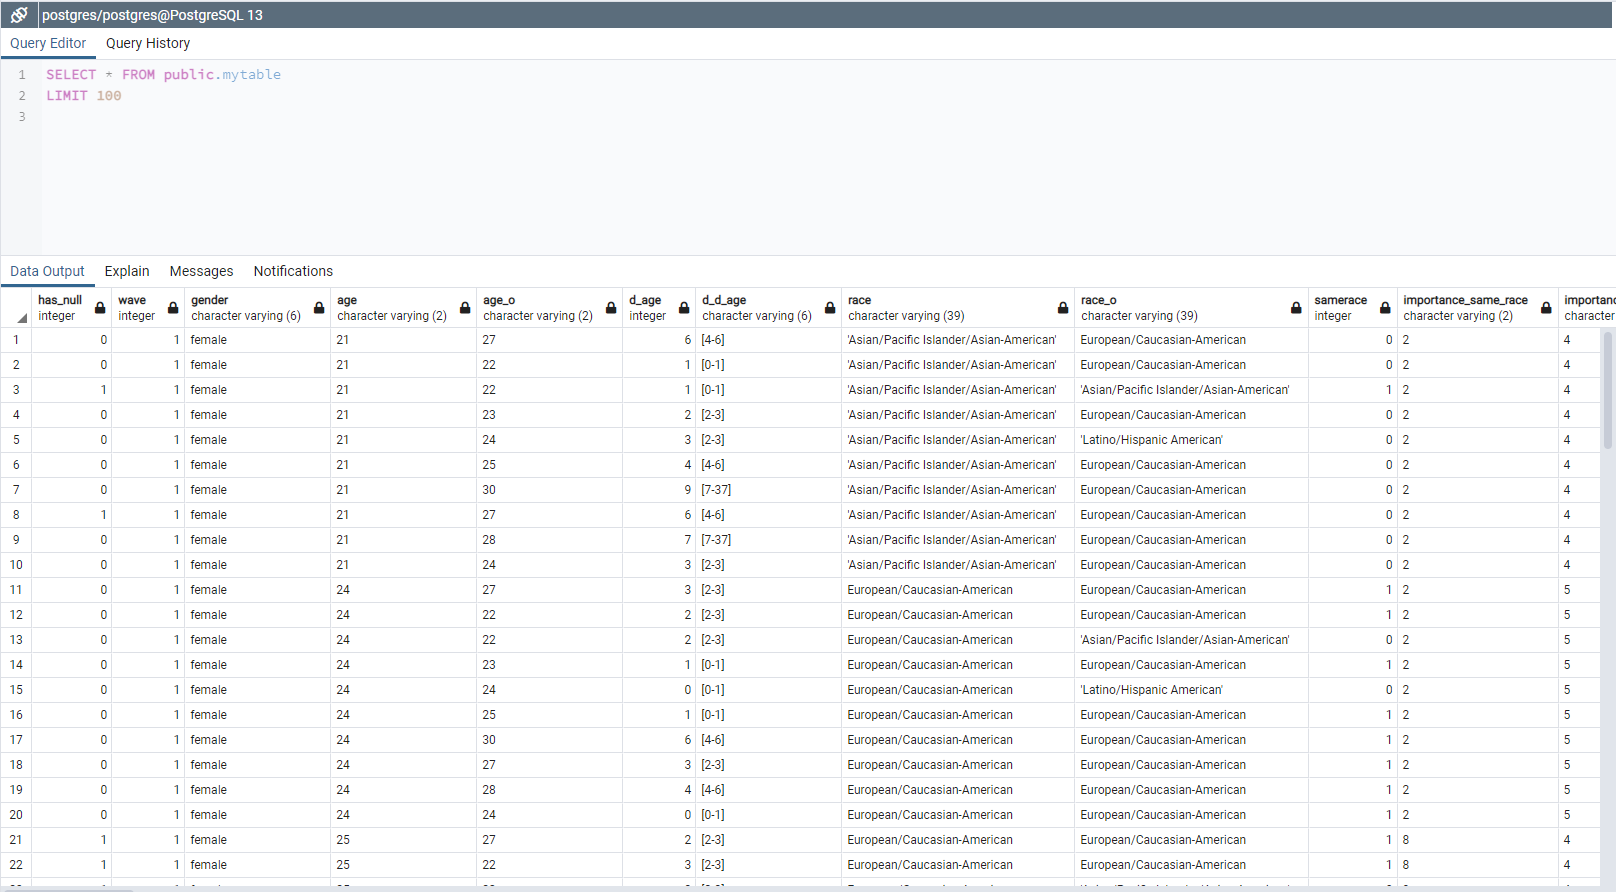
\includegraphics[scale=0.2]{bazadanych.png}
\caption{Zrzut ekranu programu PgAdmin 4 przedstawiający pierwsze kilka rzędów danych \cite{database}.} 
\end{figure}

%\begin{figure}
%\includegraphics{}
%\caption{}
%\end{figure}

% DONE
% Krótki opis bazy danych wybranej do podsumowywania, źródło, opis treści,
% Liczba rekordów (min. $10\,000$ i koniecznie wszystkie tego
% samego typu), liczba atrybutów możliwych do rozmycia (min. $10$), czyli o stosunkowo dużej
% liczbie możliwych wartości. 
%Zwyczajowe wartości lingwistyczne nadawane wybranym
% atrybutom oraz dlaczego istnieje zwyczaj, zapotrzebowanie/inne powody
% ,,przekałdania'' tych danych na język
% naturalny (a nie formalny) 
% opis użyteczność/zastosowania. 

% DONE ale do sprawdzenia czy bardziej to dodać
% Dodać opis możliwych wartości atrybutów

% TO DO
% Realizacja bazy w wybranym DBMS. Rysunek lub tabela (fragment).

\subsection{Zmienne lingwistyczne (atrybuty/własności obiektów)}

Poniżej zostały przedstawione wzory i wykresy przedstwiające poszczególne zmienne lingwistyczne. \( \mu_z(x) \) oznacza wartość funkcji przynależności zmiennej lingwistycznej \(z\) dla danego atrybutu zbioru danych zależnie od wartości x:

\begin{enumerate}
  \item age

      \begin{equation}
        \mu_{teenager} =
          \begin{cases}
            1 & \text{dla } x \in [16,18] \\
            -0.25x +5 & \text{ dla } x \in [18,20]
          \end{cases}  
      \end{equation}

      \begin{equation}
        \mu_{young} =
        \begin{cases}
            0.2x-3.4 & \text{ dla } x \in [17,22]  \\
            1 & \text{ dla } x \in [23,28] \\
            -0.5x + 15 & \text{ dla } x \in [28,30]
          \end{cases}
      \end{equation}

      \begin{equation}
        \mu_{\text{in middle age}} =
                \begin{cases}
            0.125x-3.375 & \text{ dla } x \in [28,34]  \\
            1 & \text{ dla } x \in [35,40] \\
            -0.25x + 11 & \text{ dla } x \in [40,44]
          \end{cases}
      \end{equation} 

      \begin{equation}
        \mu_{\text{in the prime of age}} =
        \begin{cases}
            0.2x-8 & \text{ dla } x \in [40,45]  \\
            1 & \text{ dla } x \in [45,49] \\
            -x + 50 & \text{ dla } x \in [19,50]
          \end{cases}
      \end{equation} 

      \begin{equation}
        \mu_{old} =
        \begin{cases}
            0.2x-9 & \text{ dla } x \in [45,50]  \\
            1 & \text{ dla } x \in [50,65] \\
          \end{cases}
      \end{equation} 

      \begin{figure}[H]
      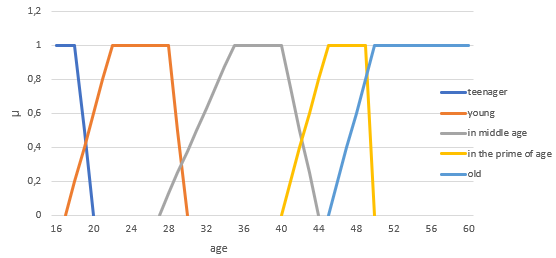
\includegraphics{fp_av2.png}
      \caption{Wykres funkcji przynależności dla atrybutu \(age\).}
      \end{figure}

  \item d\_age 

  \begin{equation}
    \mu_{none} =
      \begin{cases}
        1 & \text{dla } x =0 \\
        -x +1 & \text{ dla } x \in [0,1]
      \end{cases}  
  \end{equation}

  \begin{equation}
  \mu_{tiny} =
      \begin{cases}
        0.33x-0.33 & \text{dla } x \in [1,3] \\
        1 & \text{ dla } x=3\\
        -0.5x+3 & \text{dla } x \in [3,5] 
      \end{cases}  
  \end{equation}

  \begin{equation}
    \mu_{small} =
        \begin{cases}
          0.25x-0.75 & \text{dla } x \in [3,7] \\
          1 & \text{ dla } x=7\\
          -0.33x+3.33 & \text{dla } x \in [7,10] 
        \end{cases}  
    \end{equation}

    \begin{equation}
      \mu_{average} =
          \begin{cases}
            0.125x-1.125 & \text{dla } x \in [9,17] \\
            1 & \text{ dla } x\in [17,19]\\
            -0.25x+5.75 & \text{dla } x \in [19,23] 
          \end{cases}  
      \end{equation}

      \begin{equation}
        \mu_{significant} =
            \begin{cases}
              0.2x-3 & \text{dla } x \in [15,19] \\
              1 & \text{ dla } x\in [19,22]\\
              -0.1x+3.2 & \text{dla } x \in [22,32] 
            \end{cases}  
        \end{equation}
        \begin{equation}
          \mu_{huge} =
              \begin{cases}
                0.2x-6 & \text{dla } x \in [30,35] \\
                1 & \text{ dla } x\in [35,45]\\
              \end{cases}  
          \end{equation}
    \begin{figure}[H]
    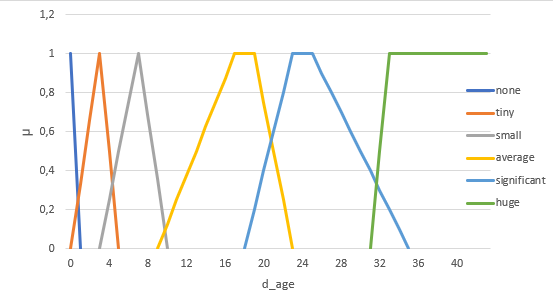
\includegraphics{fp_da.png}
    \caption{Wykres funkcji przynależności dla atrybutu \(d\_age\).}
    \end{figure}

  \item importance\_same\_race

   \begin{equation}
      \mu_{\text{nieistotne}} =
        \begin{cases}
          1 & \text{dla } x =0 \\
          -x +1 & \text{ dla } x \in [0,1]
        \end{cases}  
    \end{equation}

    \begin{equation}
      \mu_{\text{mało istotne}} =
        \begin{cases}
          x-1 & \text{dla } x \in [1,2] \\
          1 & \text{ dla } x =2 \\
          -x+3 & \text{ dla } x \in [2,3]       
        \end{cases}  
    \end{equation}

    \begin{equation}
      \mu_{\text{średnio ważne}} =
        \begin{cases}
          x-2 & \text{dla } x \in [2,3] \\
          1 & \text{ dla } x \in [3,4] \\
          -x+5 & \text{ dla } x \in [4,5]       
        \end{cases}  
    \end{equation}

    \begin{equation}
      \mu_{\text{przeciętne}} =
        \begin{cases}
          x-4 & \text{dla } x \in [4,5] \\
          1 & \text{ dla } x =5 \\
          -x+6 & \text{ dla } x \in [5,6]       
        \end{cases}  
    \end{equation}

    \begin{equation}
      \mu_{\text{znaczące}} = e^{-{(x-6)}^2}, \text{ dla } x \in [5,7]
    \end{equation}

    \begin{equation}
      \mu_{\text{ważne}} = e^{-(\frac{x-9}{1.5})^2}, \text{ dla } x \in [7,10]
    \end{equation}

      \begin{figure}[H]
      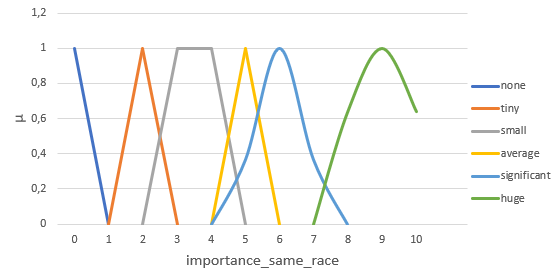
\includegraphics{fp_isrv2.png}
      \caption{Wykres funkcji przynależności dla atrybutu \(importance\_same\_race\).}
      \end{figure}

  

  \item importance\_same\_religion 
    \begin{equation}
      \mu_{\text{none}} =
        \begin{cases}
          1 & \text{dla } x =0 \\
          -x +1 & \text{ dla } x \in [0,1]
        \end{cases}  
    \end{equation}

    \begin{equation}
      \mu_{\text{tiny}} =
        \begin{cases}
          x-1 & \text{dla } x \in [1,2] \\
          1 & \text{ dla } x =2 \\
          -x+3 & \text{ dla } x \in [2,3]       
        \end{cases}  
    \end{equation}

    \begin{equation}
      \mu_{\text{small}} =
        \begin{cases}
          x-2 & \text{dla } x \in [2,3] \\
          1 & \text{ dla } x \in [3,4] \\
          -x+5 & \text{ dla } x \in [4,5]       
        \end{cases}  
    \end{equation}

    \begin{equation}
      \mu_{\text{average}} =
        \begin{cases}
          x-4 & \text{dla } x \in [4,5] \\
          1 & \text{ dla } x =5 \\
          -x+6 & \text{ dla } x \in [5,6]       
        \end{cases}  
    \end{equation}

    \begin{equation}
      \mu_{\text{significant}} = e^{-{(x-6)}^2}, \text{ dla } x \in [5,7]
    \end{equation}

    \begin{equation}
      \mu_{\text{huge}} = e^{-(\frac{x-9}{1.5})^2}, \text{ dla } x \in [7,10]
    \end{equation}

      \begin{figure}[H]
      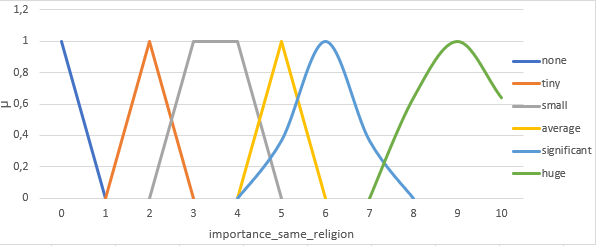
\includegraphics{fp_rel.png}
      \caption{Wykres funkcji przynależności dla atrybutu \(importance\_same\_religion\).}
      \end{figure}
  

  \item pref\_o\_intelligence
  \begin{equation}
    \mu_{stupid} =
      \begin{cases}
        1 & \text{ dla } x \in [0 ,1] \\
        -0.5x+1.5 & \text{ dla } x \in [1,3]       
      \end{cases}  
  \end{equation}

  \begin{equation}
    \mu_{\text{not very intelligent}} =
      \begin{cases}
        0.33x-0.66 & \text{ dla } x \in [2,5]\\
        1 & \text{ dla } x \in [5,12] \\
        -0.25x+4 & \text{ dla } x \in [12,16]       
      \end{cases}  
  \end{equation}

  \begin{equation}
    \mu_{average} =
      \begin{cases}
        0.166x-2.33 & \text{ dla } x \in [14,20]\\
        1 & \text{ dla } x \in [20,30] \\
        -0.2x+7 & \text{ dla } x \in [30,35]       
      \end{cases}  
  \end{equation}

  \begin{equation}
    \mu_{intelligent} =
      \begin{cases}
        0.083x-2.67 & \text{ dla } x \in [32,44]\\
        1 & \text{ dla } x \in [44,58] \\
        -0.16x+10.3 & \text{ dla } x \in [58,64]       
      \end{cases}  
  \end{equation}

  \begin{equation}
    \mu_{genius} =
      \begin{cases}
        0.2x-11.4 & \text{ dla } x \in [57,62] \\
        1 & \text{ dla } x \in [62,67] \\   
      \end{cases}  
  \end{equation}
  
  \begin{figure}[H]
    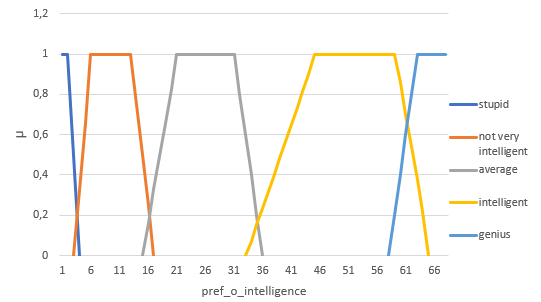
\includegraphics{fp_poiv2.png}
    \caption{Wykres funkcji przynależności dla atrybutu \(pref\_o\_intelligence\).}
    \end{figure}

  \item pref\_o\_ambitious
  \begin{equation}
    \mu_{\text{not ambitious}} = e^{-(\frac{x-6}{8})^2}, \text{ dla } x \in [0,24]
  \end{equation}

  \begin{equation}
    \mu_{\text{moderately ambitious}} = e^{-(\frac{x-30}{12})^2}, \text{ dla } x \in [5,54]
  \end{equation}

  \begin{equation}
    \mu_{\text{very ambitious}} = e^{-(\frac{x-45}{5})^2}, \text{ dla } x \in [30,55]
  \end{equation}
  
  \begin{figure}[H]
    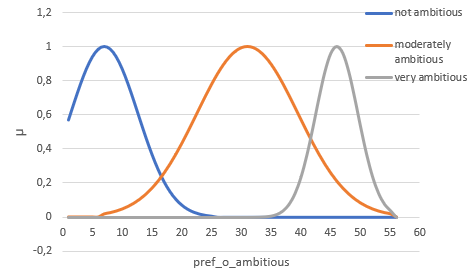
\includegraphics{fp_poav2.png}
    \caption{Wykres funkcji przynależności dla atrybutu \(pref\_o\_ambitious\).}
    \end{figure}
  
  \item tvsports 
  \begin{equation}
    \mu_{\text{not interested}} =
      \begin{cases}
        1 & \text{ dla } x \in [0,2] \\
        -0.33x+1.67 & \text{ dla } x \in [2,5]       
      \end{cases}  
  \end{equation}

  \begin{equation}
    \mu_{neutral} =
      \begin{cases}
        0.5x-1 & \text{ dla } x \in [2,4]\\
        1 & \text{ dla } x=4 \\
        -0.33x+2.34 & \text{ dla } x \in [4,7]       
      \end{cases}  
  \end{equation}

  \begin{equation}
    \mu_{\text{moderately interested}} =
      \begin{cases}
        0.5x-2 & \text{ dla } x \in [4,6]\\
        1 & \text{ dla } x \in [6,8] \\
        -x+9 & \text{ dla } x \in [8,9]       
      \end{cases}  
  \end{equation}

  \begin{equation}
    \mu_{interested} =
      \begin{cases}
        x-8 & \text{ dla } x \in [8,9]\\
        1 & \text{ dla } x =9 \\
        -0.5x+5.5 & \text{ dla } x \in [9,11]       
      \end{cases}  
  \end{equation}

  \begin{equation}
    \mu_{passionate} =
      \begin{cases}
        0.5x-4.5 & \text{ dla } x \in [9,11]\\
        1 & \text{ dla } x \in [11,12] \\
     
      \end{cases}  
  \end{equation}

  \begin{figure}[H]
    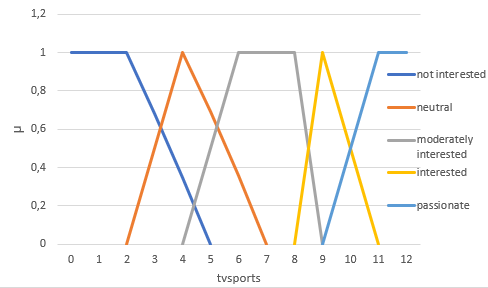
\includegraphics{fp_tv2.png}
    \caption{Wykres funkcji przynależności dla atrybutu \(tvsports\).}
    \end{figure}

  \item expected\_num\_interested\_in\_me
  
  \begin{equation}
    \mu_{none} =
      \begin{cases}
        1 & \text{ dla } x \in [0,1] \\
        0.5x+1.5  & \text{ dla } x \in [1,3]
      \end{cases}  
  \end{equation} 

  \begin{equation}
    \mu_{few} =
      \begin{cases}
        0.5x-0.5 & \text{ dla } x \in [1,3] \\
        1 & \text{ dla } x \in [3,4] \\
        -x+5  & \text{ dla } x \in [4,6]
      \end{cases}  
  \end{equation}
  
  \begin{equation}
    \mu_{not many} =
      \begin{cases}
        x-4 & \text{ dla } x \in [4,5] \\
        1 & \text{ dla } x =5 \\
        0.5x+3.5  & \text{ dla } x \in [5,7]
      \end{cases}  
  \end{equation}

  \begin{equation}
    \mu_{some} =
      \begin{cases}
        x-6 & \text{ dla } x \in [6,7] \\
        1 & \text{ dla } x =7 \\
        -x+4  & \text{ dla } x \in [7,8]
      \end{cases}  
  \end{equation}
  
  \begin{equation}
    \mu_{many} =
      \begin{cases}
        x+8 & \text{ dla } x \in [7,9] \\
        1 & \text{ dla } x =9 \\
        -x+10  & \text{ dla } x \in [9,11]
      \end{cases}  
  \end{equation}

  \begin{equation}
    \mu_{a lot} =
      \begin{cases}
        0.5x-4.5 & \text{ dla } x \in [8,11] \\
        1 & \text{ dla } x \in [11,12]
      \end{cases}  
  \end{equation}

  \begin{figure}[H]
    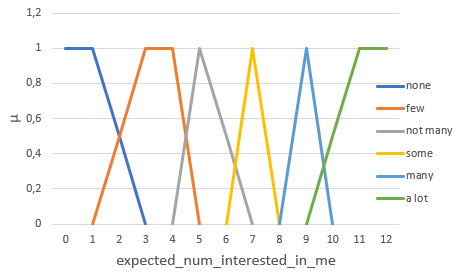
\includegraphics{fp_enimv2.png}
    \caption{Wykres funkcji przynależności dla atrybutu \(expected\_num\_interested\_in\_me\).}
    \end{figure}

  \item guess\_prob\_liked
  \begin{equation}
    \mu_{none} =
      \begin{cases}
        1 & \text{ dla } x \in [0,1] \\
        -x+2  & \text{ dla } x \in [1,2]
      \end{cases}  
  \end{equation}

  \begin{equation}
    \mu_{tiny} =
      \begin{cases}
        0.5x-0.5 & \text{ dla } x \in [1,3] \\
        1 & \text{ dla } x =3 \\
        -x+4  & \text{ dla } x \in [3,4]
      \end{cases}  
  \end{equation}

  \begin{equation}
    \mu_{small} =
      \begin{cases}
        0.5x-1.5 & \text{ dla } x \in [3,5] \\
        1 & \text{ dla } x =5 \\
        -x+6  & \text{ dla } x \in [5,6]
      \end{cases}  
  \end{equation}

  \begin{equation}
    \mu_{significant} =
      \begin{cases}
        0.34x-1.67 & \text{ dla } x \in [5,8] \\
        1 & \text{ dla } x \in [8,9] \\
        -x+9  & \text{ dla } x \in [9,10]
      \end{cases}  
  \end{equation}

  \begin{equation}
    \mu_{huge} =
      \begin{cases}
        0.5x-4.5 & \text{ dla } x \in [9,11] \\
        1 & \text{ dla } x \in [11,12] \\
      \end{cases}  
  \end{equation}

  \begin{figure}[H]
    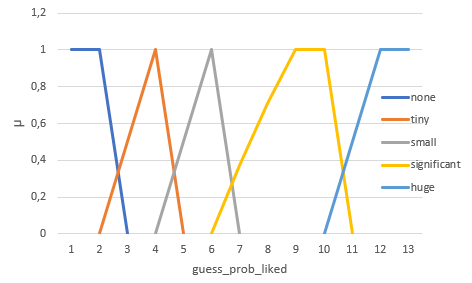
\includegraphics{fp_gplv2.png}
    \caption{Wykres funkcji przynależności dla atrybutu \(guess\_prob\_liked \).}
    \end{figure}

  \item funny
  \begin{equation}
    \mu_{boring} =
      \begin{cases}
        1 & \text{ dla } x \in [0,2] \\
        -0.5x-1.5 & \text{ dla } x \in [2,3] 
      \end{cases}  
  \end{equation}
 
  \begin{equation}
    \mu_{\text{a little bit boring}} =
      \begin{cases}
        0.33x-0.34 & \text{ dla } x \in [1,4] \\
        1 & \text{ dla } x \in [4,5] \\
        -x+6 & \text{ dla } x \in [5,6] 
      \end{cases}  
  \end{equation}
  
  \begin{equation}
    \mu_{entertaining} =
      \begin{cases}
        x-5 & \text{ dla } x \in [5,6] \\
        1 & \text{ dla } x \in [6,7] \\
        -0.34x-3.34 & \text{ dla } x \in [7,10] 
      \end{cases}  
  \end{equation}

  \begin{equation}
    \mu_{funny} =
      \begin{cases}
        x-9 & \text{ dla } x \in [9,10] \\
        1 & \text{ dla } x \in [10,13] \\
        
      \end{cases}  
  \end{equation}

  \begin{figure}[H]
    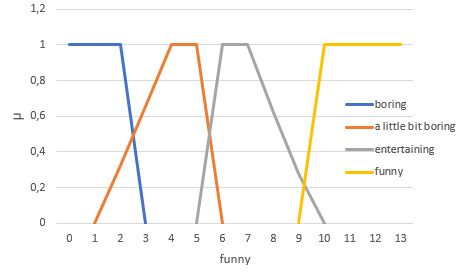
\includegraphics{fp_fv2.png}
    \caption{Wykres funkcji przynależności dla atrybutu \(funny\).}
    \end{figure}

  \item sincere
  
  \begin{equation}
    \mu_{duplicitous} =
      \begin{cases}
        1 & \text{ dla } x \in [0,2] \\
        -0.34x+2 & \text{ dla } x \in [2,6] \\
      \end{cases}  
  \end{equation}

  \begin{equation}
    \mu_{insincere} =  e^{-(\frac{x-7}{2})^2}, dla x \in [4,11]
  \end{equation}

  \begin{equation}
    \mu_{sincere} =
      \begin{cases}
        0.34x-2.67 & \text{ dla } x \in [8,11] \\
        1 & \text{ dla } x \in [11,13] \\
      \end{cases}  
  \end{equation}

  
  \begin{figure}[H]
    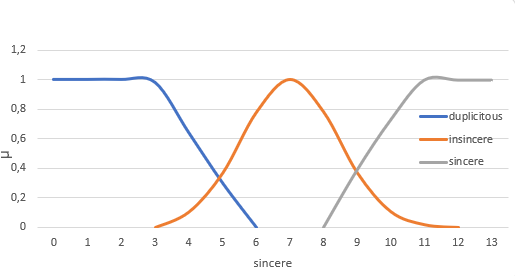
\includegraphics{fp_sv2.png}
    \caption{Wykres funkcji przynależności dla atrybutu \(sincere\).}
    \end{figure}

\end{enumerate}


%Zmienne lingwistyczne dla wybranych 10 atrybutów z bazy danych, przedstawione w
%formie wykresów funkcji przynależności i wzorów analitycznych, wymienione etykiety oraz objaśnione wszystkie
%symbole ułatwiające czytelnikowi ich zrozumienie \cite{zadrozny06}. {\bf Zbędne jest
%cytowanie definicji}. Konieczne {\bf precyzyjnie podane przestrzenie rozważań każdej
%zmiennej lingwistycznej}, wzory i wykresy dla każdej wartości/etykiety.

\subsection{Kwantyfikatory lingwistyczne (liczności obiektów)}

Poniżej zostały przedstawione wzory i wykresy przedstwiające poszczególne kwantyfikatory lingwistyczne, zarówno względne jak i absolutne. 
\( \mu_z(x) \) oznacza wartość funkcji przynależności kwantyfikatora lingwistycznego \(z\) dla danego atrybutu zbioru danych zależnie od wartości x:

 \begin{equation}
    \mu_{\text{Almost none of}} = 
    \begin{cases}
        1 & \text{ dla } x \in [0,0.006] \\
        2 - 0.02x & \text{ dla } x \in [0.006,0.012] \\
      \end{cases}
  \end{equation}

  \begin{equation}
    \mu_{\text{Some of}} =
      \begin{cases}
        0.005x & \text{ dla } x \in [0,0.024] \\
        1 & \text{ dla } x \in [0.024,0.179] \\
        -0.005x & \text{ dla } x \in [0.179,0.203] \\
      \end{cases}  
  \end{equation}
  
  \begin{equation}
    \mu_{\text{Approximately 1/3 of}} = e^{-(\frac{x-0.322}{0.095})^2}, \text{ dla } x \in [0.119,0.597]
  \end{equation}

   \begin{equation}
    \mu_{\text{Around half of}} =
      \begin{cases}
        0.0025x - 9.4725 & \text{ dla } x \in [0.452,0.5] \\
        -0.0025x + 11.4725 & \text{ dla } x \in [0.5,0.548] \\
      \end{cases}  
  \end{equation}
  
  \begin{equation}
    \mu_{\text{Most of}} =
      \begin{cases}
        0.002x - 8.2 & \text{ dla } x \in [0.489,0.549] \\
        1 & \text{ dla } x \in [0.549,1] \\
      \end{cases}  
  \end{equation}
  
  \begin{equation}
    \mu_{\text{The vast majority of}} =
      \begin{cases}
        0.001x - 7.3 & \text{ dla } x \in [0.871,0.991] \\
        1 & \text{ dla } x \in [0.991,1] \\
      \end{cases}  
  \end{equation}
  
 \begin{figure}[H]
 \centering
   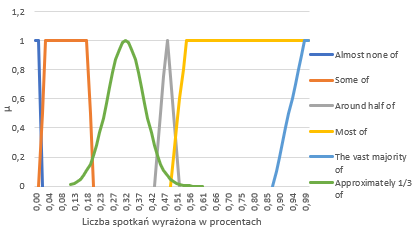
\includegraphics{wzgledne.png}
   \caption{Wykres funkcji przynależności dla kwantyfikatorów względnych użytych w zadaniu}
 \end{figure}

  
 \begin{equation}
  \mu_{\text{Less than 1000}} =
    \begin{cases}
      1 & \text{ dla } x \in [0,600] \\
      0.0034x - 3.34 & \text{ dla } x \in [600,1000] \\
    \end{cases}  
\end{equation}

\begin{equation}
  \mu_{\text{More than 1000}} = e^{-(\frac{x-1500}{500})^2}, \text{ dla } x \in [300,2700]
\end{equation}

\begin{equation}
  \mu_{\text{Approximately 3000}} =
    \begin{cases}
      0.001x - 1.6 & \text{ dla } x \in [1600,2600] \\
      1 & \text{ dla } x \in [2600,4000] \\
      0.001x +5 & \text{ dla } x \in [4000,5000] \\
    \end{cases}  
\end{equation}

\begin{equation}
  \mu_{\text{More than 5000}} =e^{-(\frac{x-5000}{1000})^2}, \text{ dla } x \in [2800,6900]
\end{equation}

\begin{equation}
  \mu_{\text{Around 8000}} =
    \begin{cases}
      0.0004x - 2.2 & \text{ dla } x \in [5500,8000] \\
      1 & \text{ dla } x \in [8000,8400] \\
    \end{cases}  
\end{equation}

 \begin{figure}[H]
  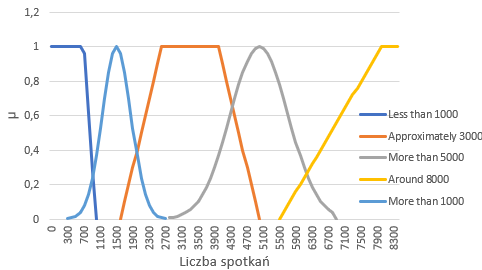
\includegraphics{absolute.PNG}
  \caption{Wykres funkcji przynależności dla kwantyfikatorów absolutnych użytych w zadaniu}
\end{figure}

%Jw. kwantyfikatory lingwistyczne -- opisane etykietami, wykresami funkcji
%przynależności i wzorami analitycznymi. Uzasadnione wiedzą dziedzinową  
%{\bf zakresy i etykiety}. Precyzyjnie podane przestrzenie rozważań każdego kwantyfikatora 
%lingwistycznego/rozmytego, wzory i wykresy dla każdej wartości/etykiety. Opisy własne z~przypisami do literatury, tak by inżynier innej specjalności zrozumiał dalszy
%opis tego konkretnego ćwiczenia/eksperymentu.  


\section{Narzędzia obliczeniowe: wybór/implementacja. Diagram UML pakietu
obliczeń rozmytych i~generatora podsumowań. Instrukcja użytkownika}

Aplikacja została napisana w technologii Java w wersji 17, z wykorzystaniem biblioteki JavaFX \cite{javafx} w celu stworzenia prostego
okienkowego interfejsu użytkownika. W celu odczytania danych zawarytch w bazie danych \cite{database} użyto Spring Framework \cite{spring}. \\

Implementacja została podzielona na dwa moduły warstwy logiki i widoku, wykorzystany został wzorzec projektowy Model View Controler. Z kolei cześć odpowiedzialna za logikę aplikacji składa się z poszczególnych pakietów:
\begin{enumerate}
  \item functions - pakiet reprezentujący funkcje przynależności (klasa abstrakcyjna MembershipFunction i rozsrzerzające ją klasy). 
  \begin{figure}[H]
    \centering
    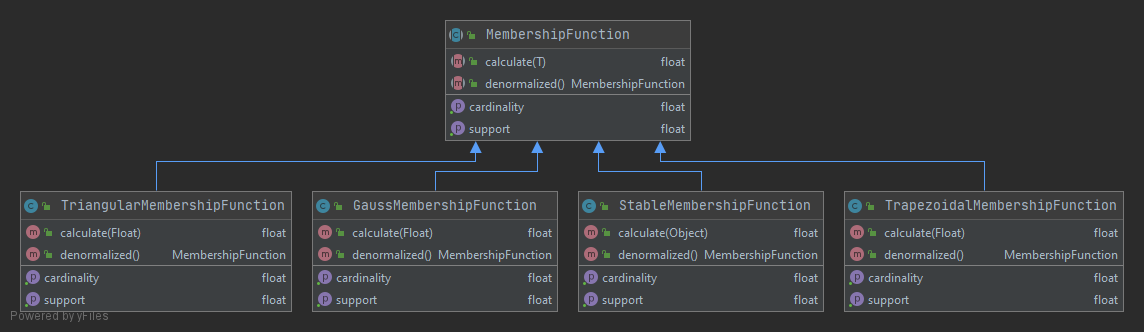
\includegraphics[scale = 0.3]{fun}
    \caption{Diagram UML pakietu \(functions\)}
  \end{figure}
  \item fuzzy - pakiet reprezentujący poszczególne elementy podsumowania, jak i samo podsumowanie lingwistyczne oraz metryki użyte to obliczeń jakości wykonywanych operacji. Zawiera międzyinnymi klasy: LinguisticVariable reprezentującą zmienną lingwistyczną, LinguisticSummary - podsumowanie lingwistyczne.
  \begin{figure}[H]    
    \centering
    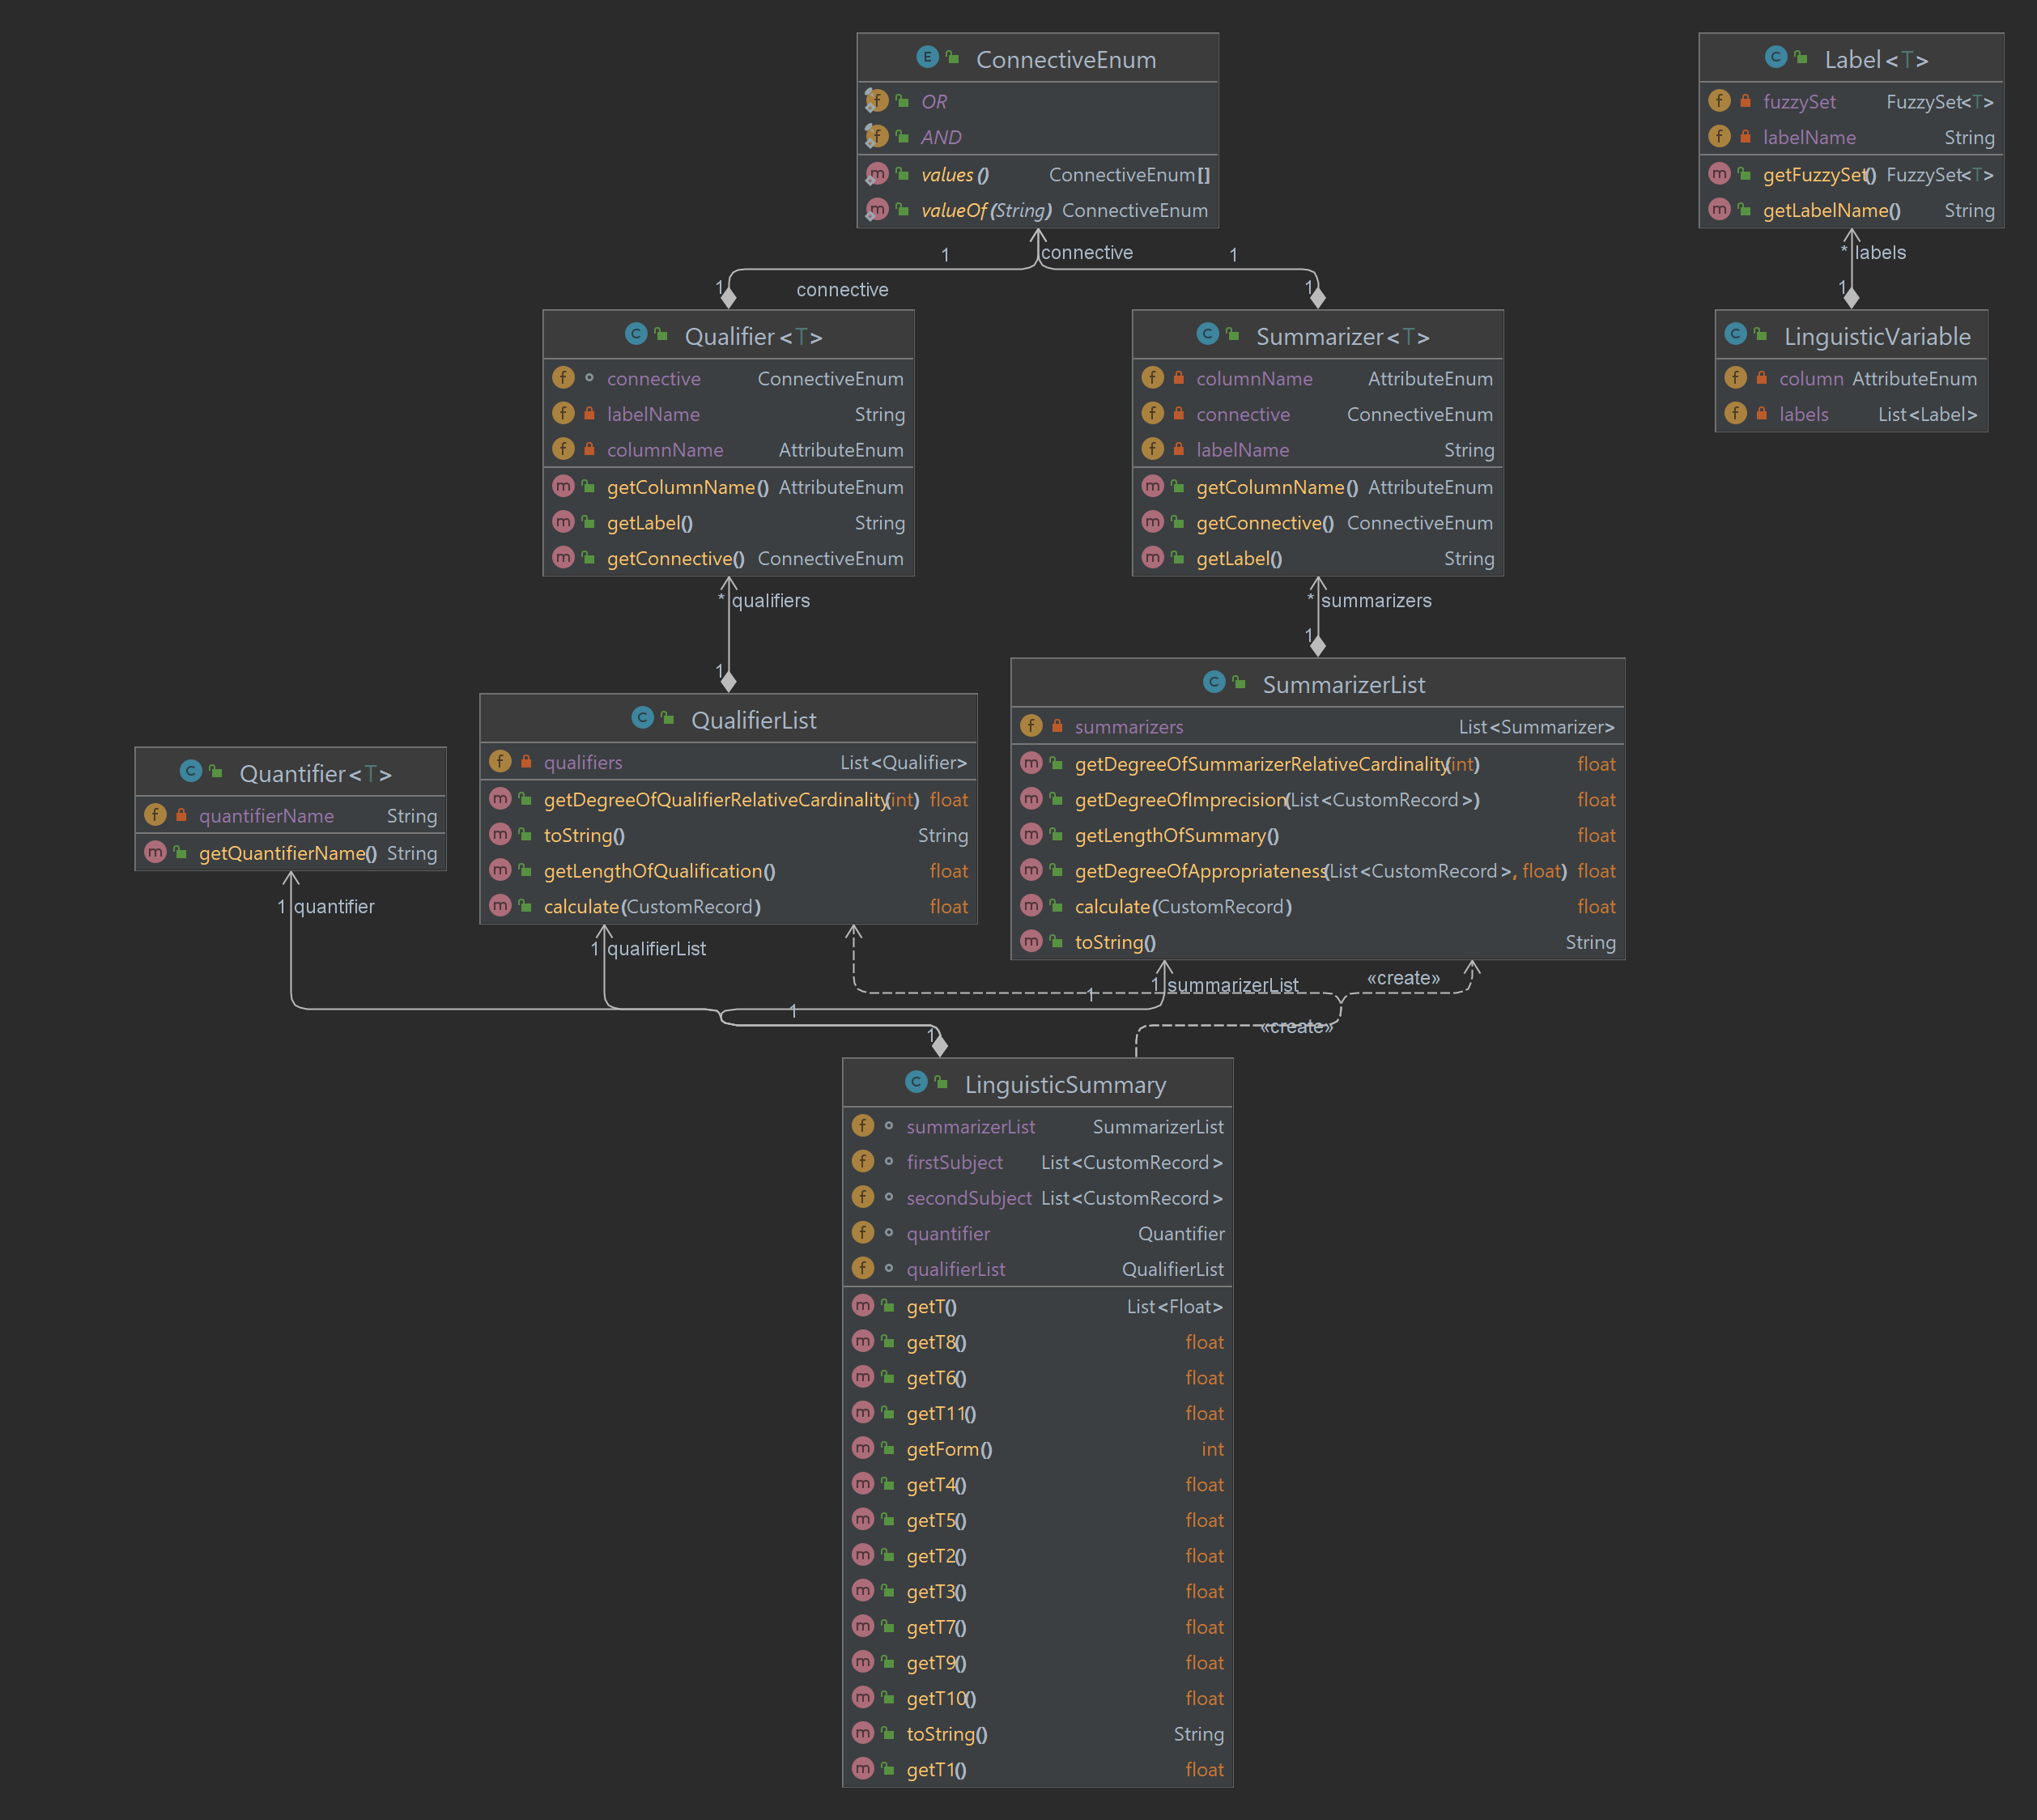
\includegraphics[scale = 0.3]{fuzzy}
    \caption{Diagram UML pakietu \(fuzzy\)}
  \end{figure}
  \item set - pakiet reprezentujący obiekt zbioru, zarówno rozmumianego w sensie klasycznym jak i rozmytym. Zawiera klase abstrakcyjną Set, która rozszerza klasę bibliioteczną ArrayList oraz rozszerzające ją klasę FuzzySet.
  \begin{figure}[H]
    \centering
    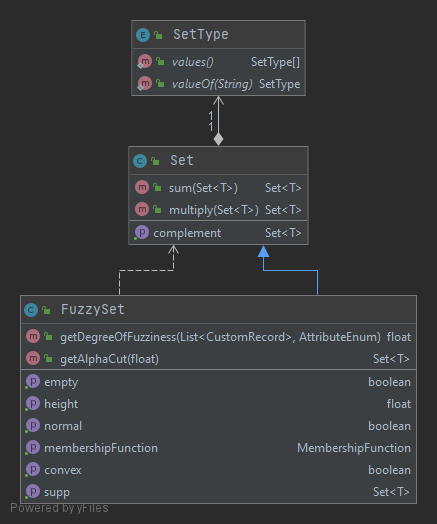
\includegraphics[scale = 0.7]{set}
    \caption{Diagram UML pakietu \(set\)}
  \end{figure}
  \item data - pakiet reprezentujący pojedyńczy rekord odczytany z bazy danych.
   \begin{figure}[H]
    \centering
    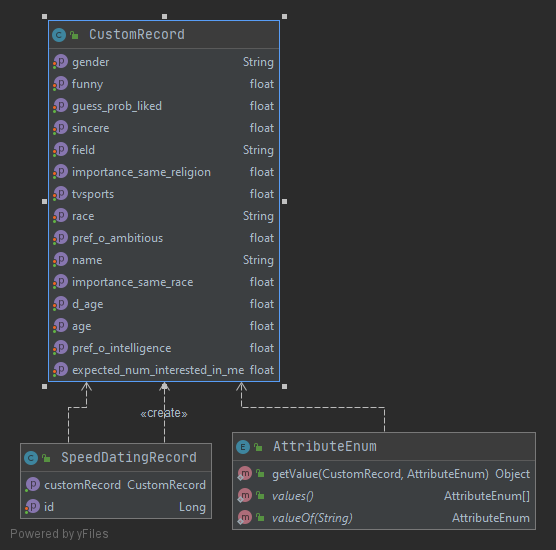
\includegraphics[scale = 0.7]{data}
    \caption{Diagram UML pakietu \(data\)}
  \end{figure}
\end{enumerate}

  \begin{figure}[H]
    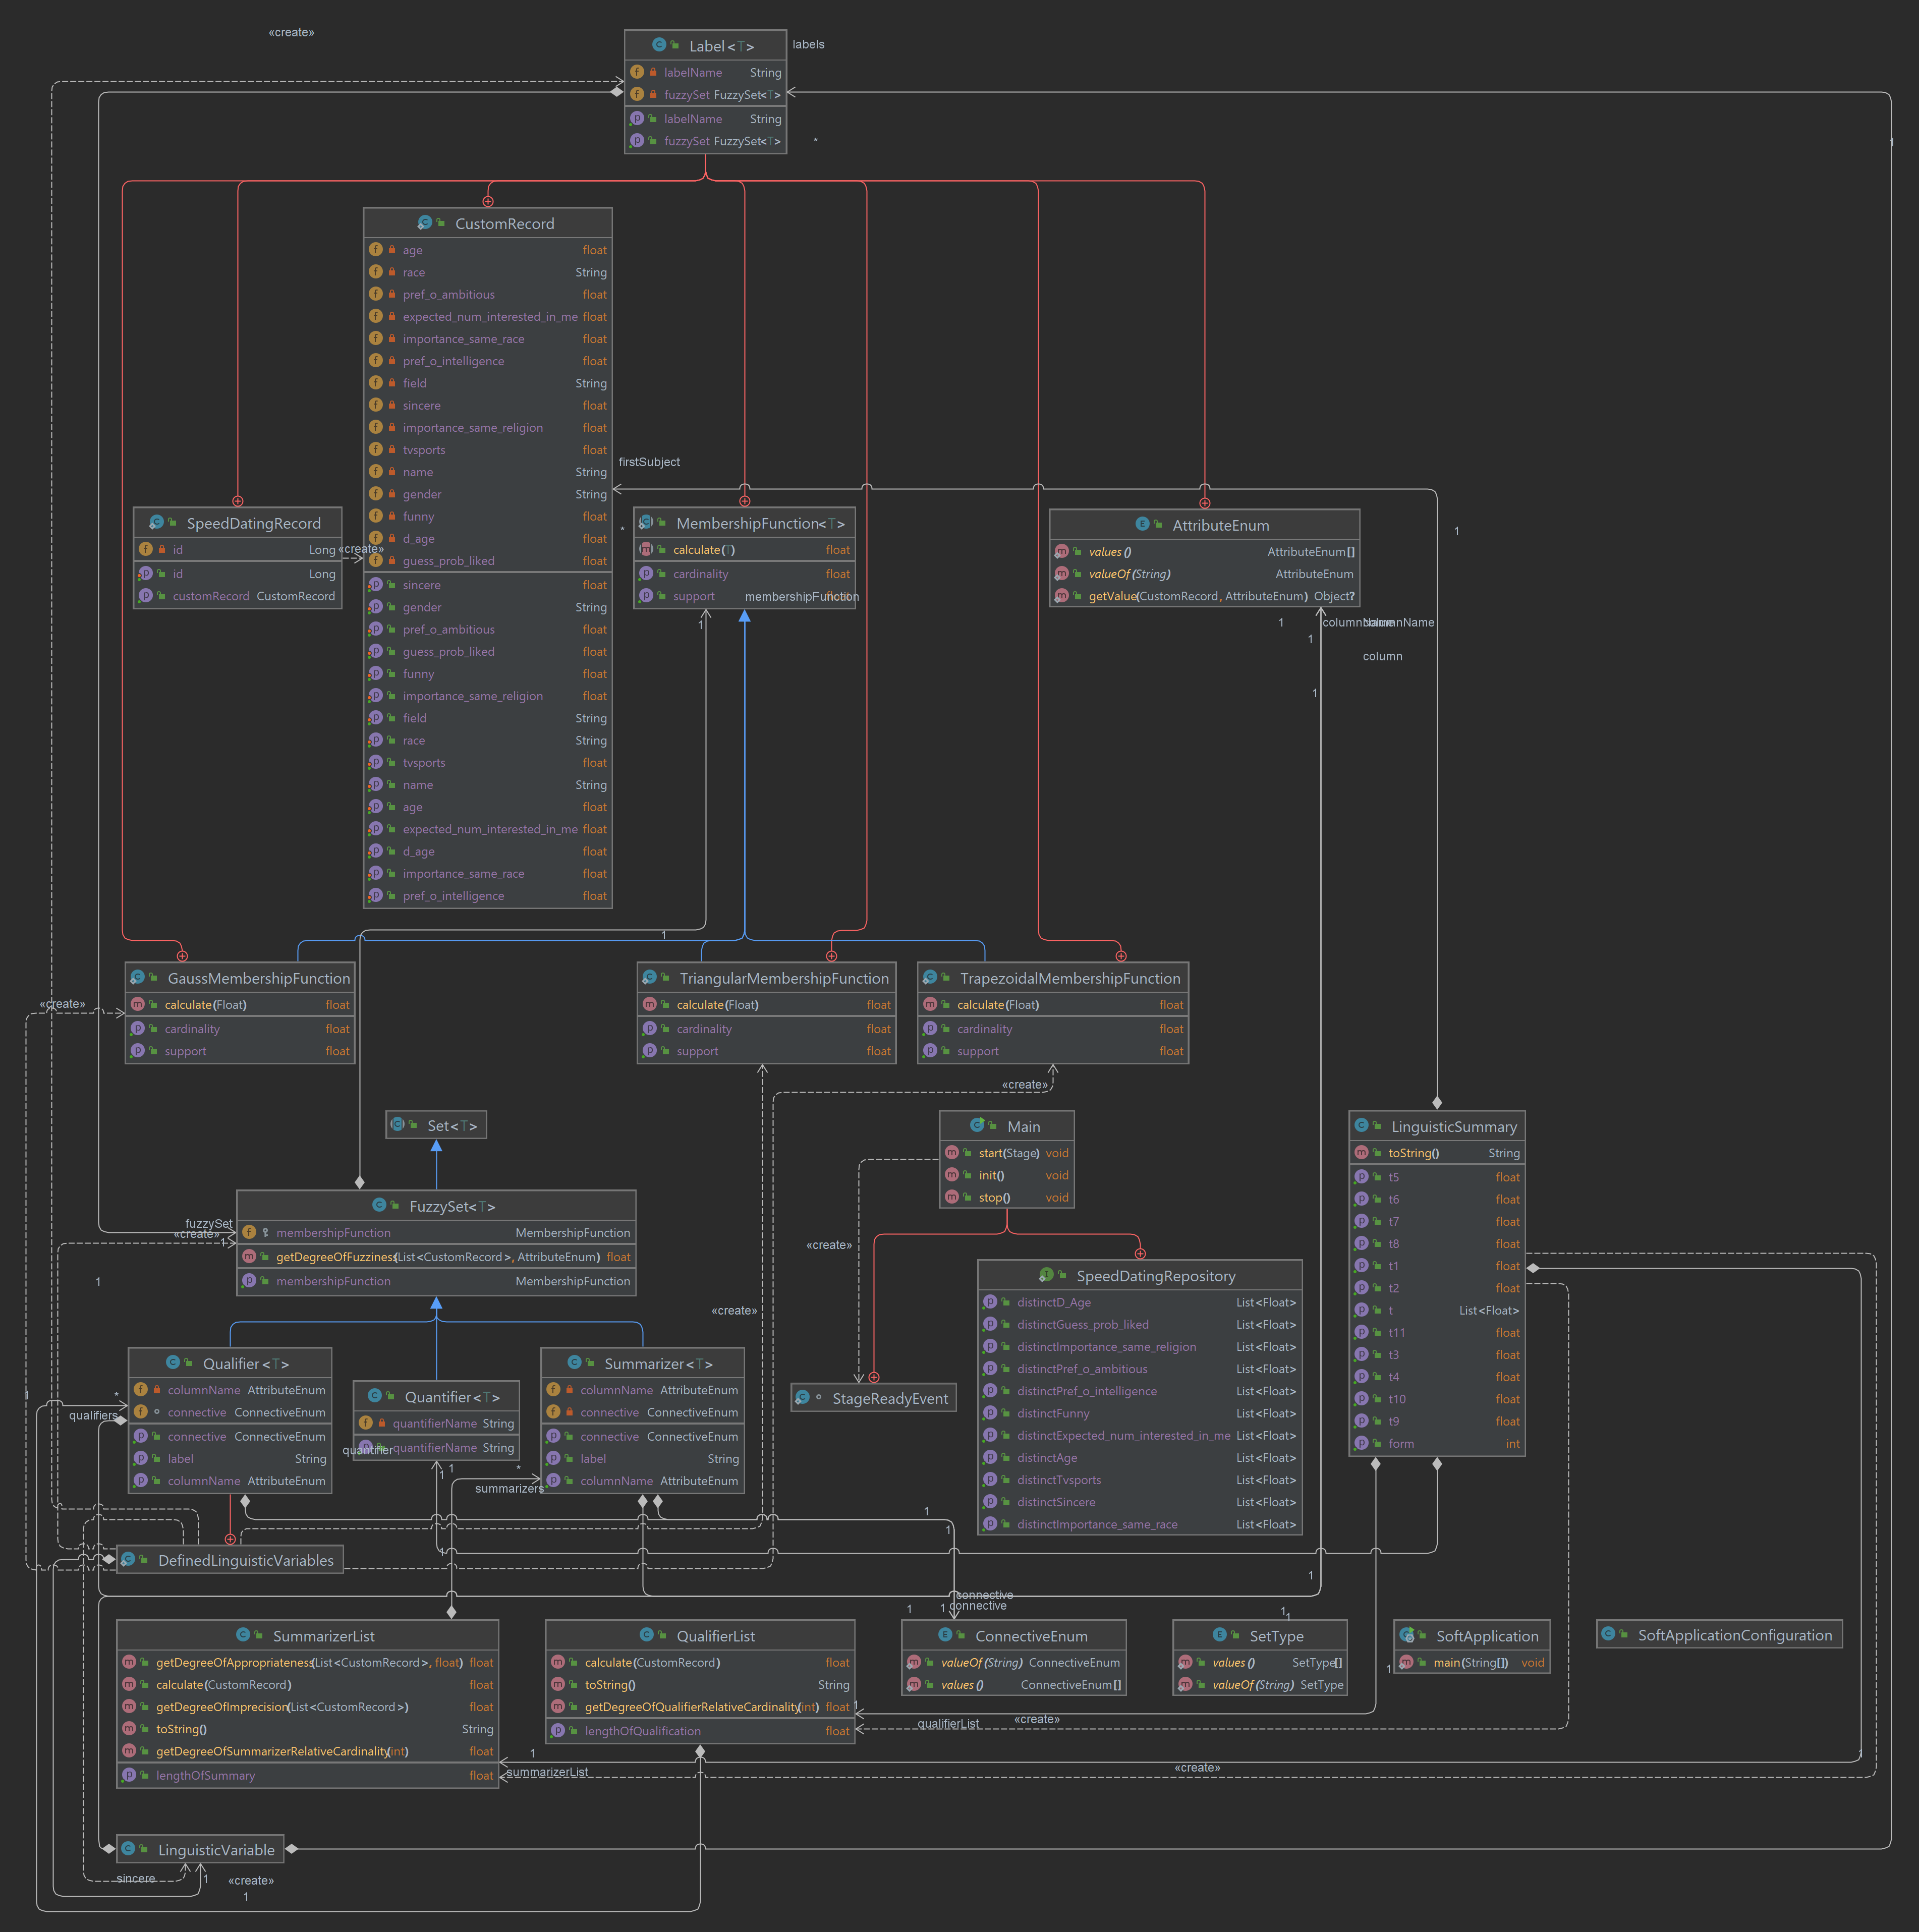
\includegraphics[scale = 0.1]{all}
    \caption{Diagram UML modułu logiki}
  \end{figure}

  Poniżej zamieszczono poszczególne widoki GUI aplikacji:
  
  \begin{figure}[H]
    \centering
    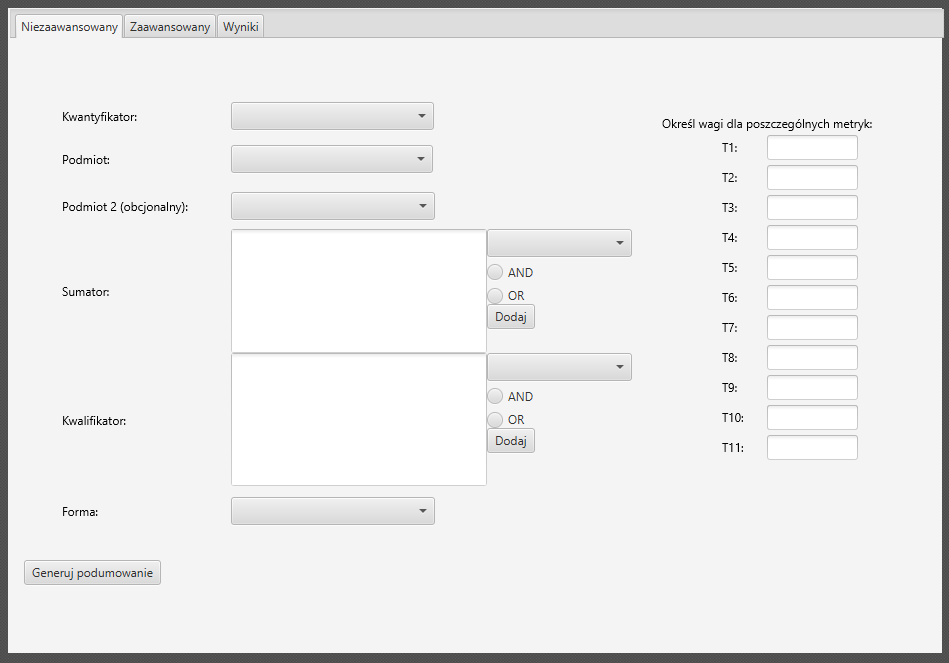
\includegraphics[scale = 0.5]{gui1}
    \caption{Widok GUI aplikacji dla użytkownika niezaawansowanego pozwalający na generowanie podsumowań poprzez wybranie między innymi kwantyfikatora, podmiotu oraz określenie wag dla poszczególnych metryk}
  \end{figure}
  
  \begin{figure}[H]
    \centering
    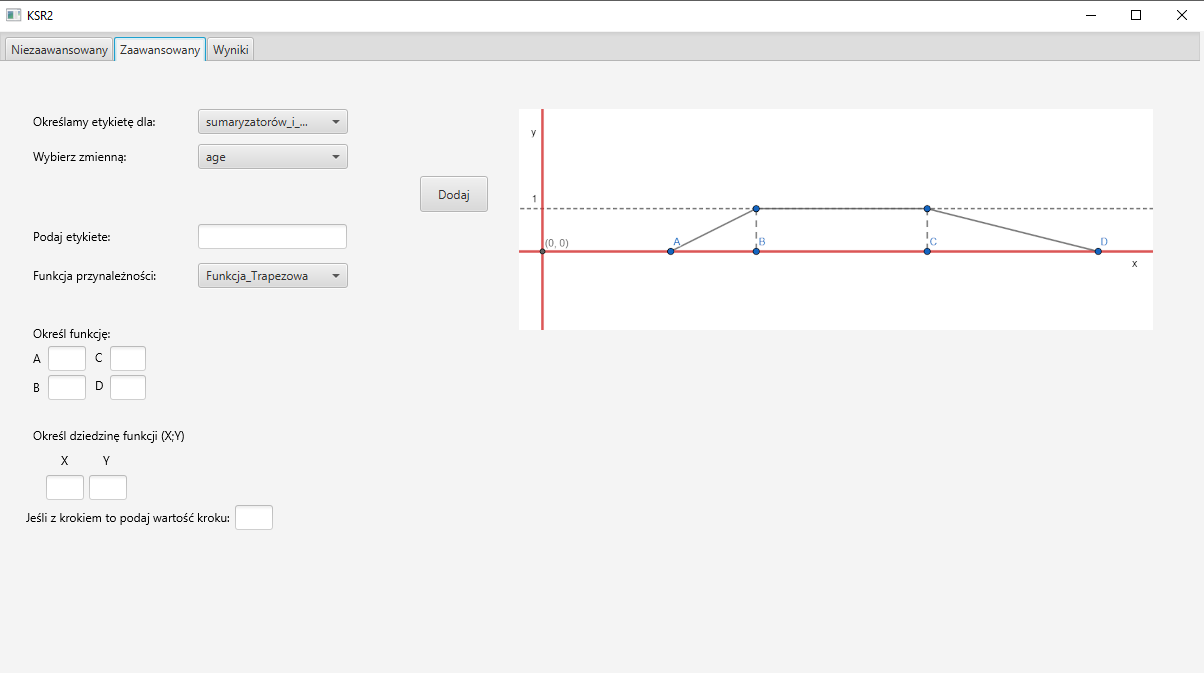
\includegraphics[scale = 0.5]{gui2}
    \caption{Widok GUI aplikacji dla użytkownika zaawansowanego pozwalający na definiowanie własnych etykiet i funckji przynależności dla nowych kwantyfikatorów, sumaryzatorów i kwalifikatorów}
  \end{figure}
  
  \begin{figure}[H]
    \centering
    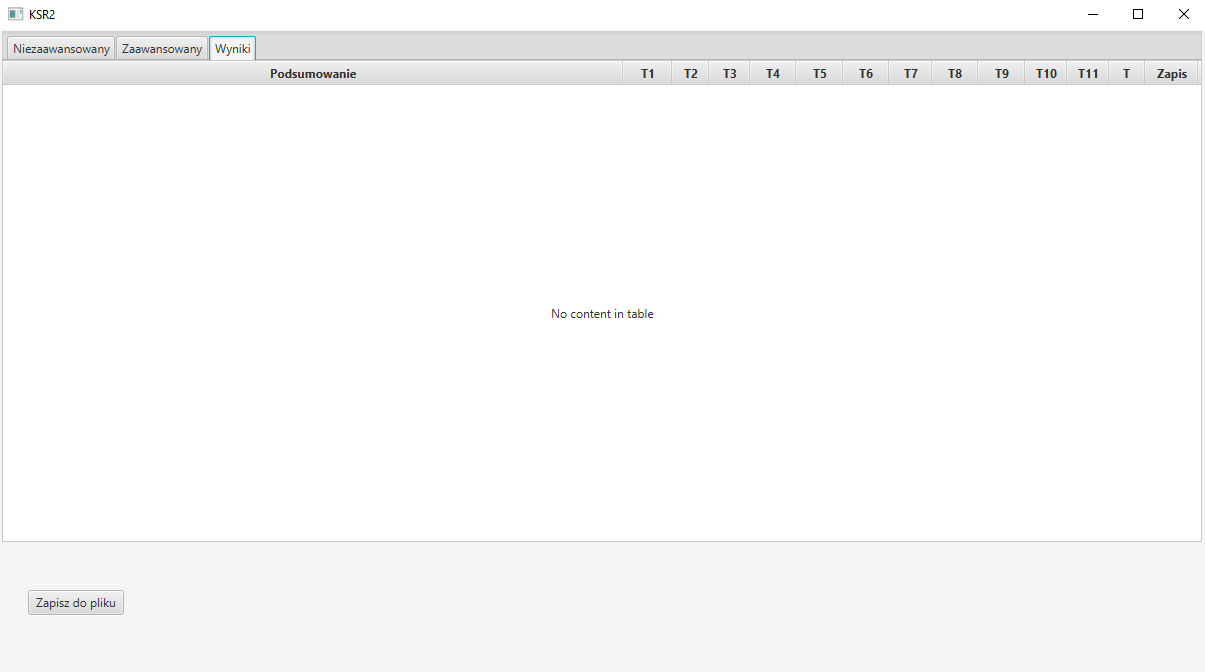
\includegraphics[scale = 0.5]{gui3}
    \caption{Widok GUI aplikacji przedstawiający wyniki podsumowań}
  \end{figure}


%\noindent {\bf Sekcja uzupełniona jako efekt zadania Tydzień 10 wg Harmonogramu Zajęć na WIKAMP KSR.}
%Diagram UML i zwięzły opis pakietu obliczeń rozmytych: źródło pakietu
%(zewnętrzny/własny/hybrydowy), przypis do literatury/źródeł.

% Krótka charakterystyka
%najważniejszych klas i podstawowych dla zadania ich metod. \\

%Diagram UML generatora podsumowań (warstwy obliczeniowej oraz interfejsu
%użytkownika). Krótki ilustrowany opis jak użytkownik może korzystać z aplikacji, w~szczególności
%wprowadzać parametry  podsumowań, odczytywać wyniki oraz definiować własne etykiety i
%kwantyfikatory.\\

%Wersja JRE i inne wymogi niezbędne do uruchomienia aplikacji przez użytkownika na własnym komputerze. 


\section{ Jednopodmiotowe podsumowania lingwistyczne. Miary jakości, podsumowanie optymalne}

\subsection{Jednopodmiotowe podsumowanie lingwistyczne w pierwszej formie}


\begin{center}
  \begin{table}[H]
    \begin{tabularx}{\textwidth}{lXc}
    
    id & Podsumowanie [$T_1$] \\ \hline 
  
    1 & Around 8000 people are/have age equals young [0.397] \\ \hline
    2 & Less than 1000 people are/have age equals teenager [1.0]\\ \hline
    3 & Some of people are/have age equals in the prime of age [0.04] \\ \hline
    4 & Approximately 3000 people are/have sincere equals insincere [0.906] \\ \hline
    5 & Less than 1000 people are/have sincere equals sincere [1.0] \\ \hline
    6 & Around half of people are/have sincere equals insincere [0.764]\\ \hline
    7 & Less than 1000 people are/have d\_age equals average [1.0] \\ \hline 
    8 & More than 5000 people are/have d\_age equals significant [0.799]\\ \hline 
    9 & Less than 1000 people are/have funny equals entertaining [0.22]\\ \hline 
    10 & Approximately 1/3 of people are/have expected\_num\_interested\_in\_me equals few [0.961] \\ \hline
    11 & Some of people are/have tvsports equals interested [0.568] \\ \hline
    12 & Less than 1000 people are/have pref\_o\_intelligence equals not very intelligent [0.307]\\ \hline
    13 & Some of people are/have pref\_o\_intelligence equals intelligent [0.849] \\ \hline
    14 & Some of people are/have pref\_o\_ambitious equals moderately ambitious [0.385] \\ \hline
    15 & Approximately 3000 people are/have pref\_o\_ambitious equals not ambitious [0.675]\\ \hline
    16 & Less than 1000 people are/have importance\_same\_religion equals significant [0.848] \\ \hline
    17 & More than 1000 people are/have importance\_same\_race equals small [0.999] \\ \hline
    18 & Some of people are/have guess\_prob\_liked equals huge [0.450] \\ \hline
    19 & Some of people are/have guess\_prob\_liked equals small and expected\_num\_interested\_in\_me equals many [0.164]\\ \hline
    20 & The vast majority of people are/have age equals teenager and pref\_o\_intelligence equals not very intelligent [0.695]\\ \hline
    21 & Approximately 3000 people are/have importance\_same\_race equals tiny and tvsports equals neutral [0.801]\\ \hline
    22 & More than 1000 people are/have importance\_same\_race equals tiny or pref\_o\_ambitious equals very ambitious [0.477]\\ \hline
  \end{tabularx}
  \caption{Tabela podsumowań lingwistycznych jednopodmiotowych w pierwszej formie.}
\end{table}
\end{center}


W poniższej tabeli zostały zawarte wartości miar jakości uzyskanego podsumowania, przy czym wagi wykorzystane do
obliczenia podsumowania optymalnego były następujęce: dla miar $T_{x} = 0.16$, gdzie $x \in {1,2,5,6,7,8}$, zaś wartości wag dla pozostałych miar są równe 0.

\begin{center}
  \begin{table}[H]
    \begin{adjustbox}{center=11cm}
    \begin{tabularx}{\textwidth}{ccccccccccccc}
    
    id & $T_1$ & $T_2$ & $T_3$ & $T_4$ & $T_5$ & $T_6$ & $T_7$ & $T_8$ & $T_9$ & $T_{10}$ & $T_{11}$ & $T$ \\ \hline 

    1 &0,397 & 0,178 & 0 & 0 & 1 & 0,656 & 0,806 & 0,999 & 0 & 0 & 0 & 0.646 \\ \hline
    2 &1 & 0,996 & 0 & 0 & 1 & 0,881 & 0,905 & 1 & 0 & 0 & 0 & 0.925\\ \hline
    3 &0,04 & 0,998 & 0 & 0 & 1 & 0,797 & 0,821 & 0,999 & 0 & 0 & 0 & 0.745 \\ \hline
    4 &0,906 & 0,264 & 0 & 0 & 1 & 0,594 & 0,714 & 1 & 0 & 0 & 0 & 0.716  \\ \hline
    5 & 1 & 0,883 & 0 & 0 & 1 & 0,881 & 0,905 & 1 & 0 & 0 & 0 & 0.91   \\ \hline  
    6 & 0,764 & 0,264 & 0 & 0 & 1 & 0,904 & 0,952 & 1 & 0 & 0 & 0 & 0.78  \\ \hline  
    7 & 1 & 0,877 & 0 & 0 & 1 & 0,881 & 0,905 & 0,999 & 0 & 0 & 0 & 0.906\\ \hline 
    8 & 0,798 & 0,094 & 0 & 0 & 1 & 0,761 & 0,894 & 0,999 & 0 & 0 & 0 & 0.728 \\ \hline 
    9 & 0,22 & 0,891 & 0 & 0 & 1 & 0,881 & 0,905 & 1 & 0 & 0 & 0 & 0.783\\ \hline 
    10 & 0,961 & 0,55 & 0 & 0 & 1 & 0,81 & 0,916 & 1 & 0 & 0 & 0 & 0.838 \\ \hline 
    11 &0,568 & 0,747 & 0 & 0 & 1 & 0,797 & 0,821 & 1 & 0 & 0 & 0 & 0.789\\ \hline
    12 & 0,307 & 0,832 & 0 & 0 & 1 & 0,881 & 0,905 & 0,999 & 0 & 0 & 0 & 0.788 \\ \hline
    13 & 0,849 & 0,965 & 0 & 0 & 1 & 0,797 & 0,821 & 0,997 & 0 & 0 & 0 & 0.869 \\ \hline
    14 & 0,385 & 0,905 & 0 & 0 & 1 & 0,797 & 0,821 & 0,999 & 0 & 0 & 0 & 0.785\\ \hline
    15 & 0,675 & 0,362 & 0 & 0 & 1 & 0,594 & 0,714 & 0,999 & 0 & 0 & 0 & 0.695 \\ \hline
    16 &0,848 & 0,921 & 0 & 0 & 1 & 0,881 & 0,905 & 1 & 0 & 0 & 0 & 0.889 \\ \hline
    17 &0,999 & 0,822 & 0 & 0 & 1 & 0,881 & 0,947 & 1 & 0 & 0 & 0 & 0.904 \\ \hline
    18 & 0,45 & 0,978 & 0 & 0 & 1 & 0,797 & 0,821 & 1 & 0 & 0 & 0 & 0.807 \\ \hline
    19 & 0,164 & 0,923 & 0 & 0 & 0,5 & 0,797 & 0,821 & 1 & 0 & 0 & 0 & 0.678 \\ \hline
    20 & 0,695 & 0,941 & 0 & 0 & 0,5 & 0,871 & 0,931 & 0,999 & 0 & 0 & 0 & 0.79\\ \hline
    21 & 0,802 & 0,805 & 0 & 0 & 0,5 & 0,594 & 0,714 & 1 & 0 & 0 & 0 & 0.706\\ \hline
    22 & 0,477 & 1 & 0 & 0 & 0,5 & 0,881 & 0,947 & 1 & 0 & 0 & 0 & 0.769\\ \hline

  \end{tabularx}
\end{adjustbox}
  \caption{Tabela wartości miar dla podsumowań lingwistycznych jednopodmiotowych w pierwszej formie.}
\end{table}
\end{center}


\subsection{Jednopodomiotowe podsumowanie lingwistyczne w drugiej formie}

\begin{center}
  \begin{table}[H]
    \begin{tabularx}{\textwidth}{lXc}
    
    id & Podsumowanie [$T_1$] \\ \hline 
  
    22 & Almost none of people having tvsports equals interested are/have d\_age equals significant [0.014] \\ \hline
    23 & Some of people having pref\_o\_ambitious equals not ambitious are/have age equals teenager [0.131] \\ \hline
    24 & Some of people having expected\_num\_interested\_in\_me equals many are/have d\_age equals significant [0.907] \\ \hline
    25 & Some of people having pref\_o\_intelligence equals not very intelligent are/have d\_age equals significant [0.451] \\ \hline
    26 & Some of people having importance\_same\_religion equals small are/have d\_age equals small [0.068] \\ \hline
    27 & Some of people having funny equals entertaining are/have d\_age equals significant [0.334]\\ \hline
    28 & Some of people having tvsports equals moderately interested are/have expected\_num\_interested\_in\_me equals none [0.725] \\ \hline 
    29 & More than 5000 people having importance\_same\_race equals small are/have pref\_o\_intelligence equals average [0.053]\\ \hline 
    30 & More than 5000 people having pref\_o\_intelligence equals average are/have funny equals funny [0.974]\\ \hline 
    31 & Approximately 3000 people having importance\_same\_religion equals average are/have sincere equals insincere [0.032]\\ \hline
    32 & Approximately 3000 people having d\_age equals average are/have tvsports equals not interested [0.679] \\ \hline
    33 & More than 1000 people having pref\_o\_intelligence equals not very intelligent are/have expected\_num\_interested\_in\_me equals some [0.982] \\ \hline
    34 & More than 1000 people having age equals young are/have tvsports equals interested [0.468] \\ \hline
    35 & More than 1000 people having funny equals entertaining are/have tvsports equals neutral [0.084] \\ \hline
    36 & More than 1000 people having importance\_same\_religion equals huge are/have importance\_same\_race equals small [0.802]\\ \hline
    37 & Less than 1000 people having importance\_same\_race equals tiny are/have funny equals entertaining [0.414] \\ \hline
    38 & Approximately 1/3 of people having importance\_same\_race equals tiny are/have d\_age equals tiny [0.143] \\ \hline
    39 & Almost none of people having importance\_same\_race equals small and importance\_same\_religion equals tiny are/have d\_age equals significant [0.682] \\ \hline
    40 & More than 5000 people having age equals in middle age and tvsports equals neutral are/have sincere equals insincere [0.313] \\ \hline
    41 & Most of People having pref\_o\_intelligence equals intelligent are/have sincere equals insincere and sincere equals insincere [0.987]\\ \hline
    42 & More than 1000 People having pref\_o\_intelligence equals average are/have sincere equals insincere and expected\_num\_interested\_in\_me equals not many [0.271]\\ \hline
    
  \end{tabularx}
  \caption{Tabela podsumowań lingwistycznych jednopodmiotowych w drugiej formie.}
\end{table}
\end{center}

W poniższej tabeli zostały zawarte wartości miar jakości uzyskanego podsumowania, przy czym wagi wykorzystane do
obliczenia podsumowania optymalnego były następujęce: dla miar $T_{x} = 0.09$, gdzie $x \in {1,2,3,4,5,6,7,8,9,10,11}$.

\begin{center}
  \begin{table}[H]
  \begin{adjustbox}{center=11cm}
    \begin{tabularx}{\textwidth}{ccccccccccccc}
    id & $T_1$ & $T_2$ & $T_3$ & $T_4$ & $T_5$ & $T_6$ & $T_7$ & $T_8$ & $T_9$ & $T_{10}$ & $T_{11}$ & $T$ \\ \hline 
    22	&	0.014	&	0.973	&	0.017	&	0.010	&	1.000	&	0.988	&	0.991	&	0.999	&	0.747	&	1.000	&	1	&	0.697	\\ \hline
23	&	0.130	&	0.996	&	0.004	&	0.000	&	1.000	&	0.797	&	0.821	&	1.000	&	0.362	&	0.999	&	1	&	0.640	\\ \hline
24	&	0.907	&	0.973	&	0.032	&	0.006	&	1.000	&	0.797	&	0.821	&	0.999	&	0.974	&	1.000	&	1	&	0.766	\\ \hline
25	&	0.451	&	0.973	&	0.019	&	0.008	&	1.000	&	0.797	&	0.821	&	0.999	&	0.832	&	0.999	&	1	&	0.711	\\ \hline
26	&	0.068	&	0.620	&	0.385	&	0.004	&	1.000	&	0.797	&	0.821	&	1.000	&	0.827	&	1.000	&	1	&	0.677	\\ \hline
27	&	0.334	&	0.973	&	0.011	&	0.016	&	1.000	&	0.797	&	0.821	&	0.999	&	0.891	&	1.000	&	1	&	0.706	\\ \hline
28	&	0.725	&	0.951	&	0.031	&	0.018	&	1.000	&	0.797	&	0.821	&	1.000	&	0.517	&	1.000	&	1	&	0.707	\\ \hline
29	&	0.053	&	0.174	&	0.816	&	0.010	&	1.000	&	0.761	&	0.894	&	0.998	&	0.822	&	1.000	&	1	&	0.678	\\ \hline
30	&	0.974	&	0.211	&	0.798	&	0.009	&	1.000	&	0.761	&	0.894	&	1.000	&	0.174	&	0.998	&	1	&	0.704	\\ \hline
31	&	0.032	&	0.264	&	0.811	&	0.075	&	1.000	&	0.594	&	0.714	&	1.000	&	0.917	&	1.000	&	1	&	0.667	\\ \hline
32	&	0.680	&	0.758	&	0.278	&	0.035	&	1.000	&	0.594	&	0.714	&	1.000	&	0.951	&	0.999	&	1	&	0.721	\\ \hline
33	&	0.982	&	0.824	&	0.174	&	0.002	&	1.000	&	0.881	&	0.947	&	1.000	&	0.832	&	0.999	&	1	&	0.778	\\ \hline
34	&	0.468	&	0.747	&	0.274	&	0.021	&	1.000	&	0.881	&	0.947	&	1.000	&	0.178	&	0.999	&	1	&	0.676	\\ \hline
35	&	0.084	&	0.667	&	0.390	&	0.057	&	1.000	&	0.881	&	0.947	&	1.000	&	0.891	&	1.000	&	1	&	0.712	\\ \hline
36	&	0.802	&	0.822	&	0.194	&	0.015	&	1.000	&	0.881	&	0.947	&	1.000	&	0.866	&	1.000	&	1	&	0.767	\\ \hline
37	&	0.414	&	0.891	&	0.100	&	0.009	&	1.000	&	0.881	&	0.905	&	1.000	&	0.886	&	1.000	&	1	&	0.728	\\ \hline
38	&	0.143	&	0.597	&	0.385	&	0.018	&	1.000	&	0.810	&	0.916	&	1.000	&	0.886	&	1.000	&	1	&	0.698	\\ \hline
39	&	0.682	&	0.973	&	0.017	&	0.010	&	1.000	&	0.988	&	0.991	&	0.999	&	0.979	&	1.000	&	0.5	&	0.732	\\ \hline
40	&	0.313	&	0.264	&	0.765	&	0.030	&	1.000	&	0.761	&	0.894	&	1.000	&	0.909	&	0.999	&	0.5	&	0.669	\\ \hline
41	&	0.987	&	0.264	&	0.740	&	0.198	&	0.500	&	0.489	&	0.519	&	1.000	&	0.965	&	0.997	&	1	&	0.689	\\ \hline
42	&	0.271	&	0.410	&	0.368	&	0.019	&	0.500	&	0.881	&	0.947	&	1.000	&	0.174	&	0.998	&	1	&	0.591	\\ \hline
  \end{tabularx}
  \end{adjustbox}
  \caption{Tabela wartości miar dla podsumowań lingwistycznych jednopodmiotowych w drugiej formie.}
\end{table}
\end{center}
 
% 
% Wyniki kolejnych eksperymentów wg punktów 2.-4. opisu projektu 2.  Listy podsumowań
% jednopodmiotowych i tabele/rankingi podsumowań dla danych atrybutów obowiązkowe i dokładnie opisane w ,,captions'' (tytułach), konieczny opis kolumn i wierszy tabel. Dla każdego podsumowania podane miary jakości oraz miara jakości podsumowania
% optymalnego. {\bf Wzorów podsumowań ani miar nie należy przepisywać ani cytować, wystarczy podać literaturę, ale
% należy skomentować co oznaczają i jaką informacje niosą wybrane miary w wybranych
% przypadkach.}\\
% \noindent {\bf Sekcja uzupełniona jako efekt zadania Tydzień 11 wg Harmonogramu Zajęć na WIKAMP KSR.}
% 
\section{Wielopodmiotowe podsumowania lingwistyczne i~ich miary jakości} 

Po pobieżnej analizie zawartości uznano, że najlepszym podziałem badanego zbioru \cite{database} jest podział bazujący na płci 
anikietowanych. Dlatego, też w wielopodmiotowych podsumowania porównaniu podlegać będą rekordy osób należących do klasy \(female\) i \(male\).

\subsection{Wielopodmiotowe podsumowania lingwistyczne w pierwszej formie}
\begin{center}
  \begin{table}[H]
    \begin{tabularx}{\textwidth}{lXc}
    
    id & Podsumowanie [$T_1$] \\ \hline 
  
    1 & Approximately 1/3 of females compared to males are/have age equals teenager [0.103] \\\hline
    2 & Around half of females compared to males are/have d\_age equals average [0.686]\\  \hline
    3 & More than 5000 females compared to Males are/have pref\_o\_ambitious equals not ambitious [0.894]\\ \hline
    4 & Around half of females compared to males are/have guess\_prob\_liked equals small [0.917]\\ \hline
    5 & Approximately 3000 females compared to males are/have expected\_num\_interested\_in\_me equals not many [0.842]\\ \hline
  \end{tabularx}
  \caption{Tabela podsumowań lingwistycznych wielopodmiotowych w pierwszej formie.}
\end{table}
\end{center}

W poniższej tabeli zostały zawarte wartości miar jakości uzyskanego podsumowania, przy czym wagi wykorzystane do
obliczenia podsumowania optymalnego były następujęce: dla miar $T_{x} = 0.09$, gdzie $x \in {1,2,3,4,5,6,7,8,9,10,11}$.

\begin{center}
  \begin{table}[H]
    \begin{tabularx}{\textwidth}{ccccccccccccc}
    id & $T_1$ & $T_2$ & $T_3$ & $T_4$ & $T_5$ & $T_6$ & $T_7$ & $T_8$ & $T_9$ & $T_{10}$ & $T_{11}$ & $T$ \\ \hline 
    1	& 0.103 & 0 & 0 & 0 & 0 & 0 & 0 & 0 & 0 & 0 & 0 & 0.009	\\ \hline
    2	&	0.686 & 0 & 0 & 0 & 0 & 0 & 0 & 0 & 0 & 0 & 0 & 0.062 \\ \hline
    3	&	0.894 & 0 & 0 & 0 & 0 & 0 & 0 & 0 & 0 & 0 & 0 & 0.081 \\ \hline
    4	& 0.917 & 0 & 0 & 0 & 0 & 0 & 0 & 0 & 0 & 0 & 0 & 0.083	\\ \hline
    5	& 0.842 & 0 & 0 & 0 & 0 & 0 & 0 & 0 & 0 & 0 & 0 & 0.077	\\ \hline
  \end{tabularx}
  \caption{Tabela wartości miar dla podsumowań lingwistycznych wielopodmiotowych w pierwszej formie.}
\end{table}
\end{center}



% Wyniki kolejnych eksperymentów wg punktów 2.-4. opisu projektu 2. Uzasadnienie i
% metoda podziału zbioru danych na rozłączne podmioty. Listy podsumowań
% wielopodmiotowych i tabele/rankingi podsumowań dla danych atrybutów obowiązkowe i
% dokładnie opisane w ,,captions'' (tytułach), konieczny opis kolumn i wierszy tabel.
% {\bf Wzorów podsumowań ani miar nie należy przepisywać ani cytować, wystarczy podać literaturę, ale
% należy skomentować co oznaczają i jaką informacje niosą wybrane miary w wybranych
% przypadkach.}Konieczne uwzględnienie wszystkich 4-ch form podsumowań wielopodmiotowych. 

% 
% ** Możliwe sformułowanie zagadnienia wielopodmiotowego podsumowania optymalnego **.\\
% \indent {** Ewentualne wyniki realizacji punktu ,,na ocenę 5.0'' wg opisu Projektu 2. i ich porównanie do wyników z
% części obowiązkowej **.}\\
% 
% \noindent {\bf Sekcja uzupełniona jako efekt zadania Tydzień 12 wg Harmonogramu Zajęć
% na WIKAMP KSR.}
% 

\section{Dyskusja, wnioski}
Dokładne interpretacje uzyskanych wyników w zależności od parametrów klasyfikacji
opisanych w punktach 3.-4 opisu Projektu 2. 
Szczególnie istotne są wnioski o charakterze uniwersalnym, istotne dla podobnych zadań. 
Omówić i wyjaśnić napotkane problemy (jeśli były). Każdy wniosek/problem powinien mieć poparcie
w przeprowadzonych eksperymentach (odwołania do konkretnych wyników: tabel i miar
jakości). Ocena które wybrane kwantyfikatory, sumaryzatory, kwalifikatory i/lub ich
miary jakości mają małe albo duże znaczenie dla wiarygodności i jakości otrzymanych
agregacji/podsumowań.  \\
\underline{Dla końcowej oceny jest to najważniejsza sekcja} sprawozdania, gdyż prezentuje poziom
zrozumienia rozwiązywanego problemu.\\

** Możliwości kontynuacji prac w obszarze logiki rozmytej i wnioskowania rozmytego, zwłaszcza w kontekście pracy inżynierskiej,
magisterskiej, naukowej, itp. **\\

\noindent {\bf Sekcja uzupełniona jako efekt zadań Tydzień 11 i Tydzień 12 wg
Harmonogramu Zajęć na WIKAMP KSR.}


\section{Braki w realizacji projektu 2.}
Wymienić wg opisu Projektu 2. wszystkie niezrealizowane obowiązkowe elementy projektu, ewentualnie
podać merytoryczne (ale nie czasowe) przyczyny tych braków. 


\begin{thebibliography}{99}
 \bibitem{niewiadomski19} A. Niewiadomski, Zbiory rozmyte typu 2. Zastosowania w reprezentowaniu informacji.  Seria „Problemy współczesnej informatyki” pod redakcją L. Rutkowskiego. Akademicka Oficyna Wydawnicza EXIT, Warszawa, 2019.
\bibitem{zadrozny06} S. Zadrożny, Zapytania nieprecyzyjne i lingwistyczne podsumowania baz danych, EXIT, 2006, Warszawa
\bibitem{niewiadomski08} A. Niewiadomski, Methods for the Linguistic Summarization of Data: Applications of Fuzzy Sets and Their Extensions, Akademicka Oficyna Wydawnicza EXIT, Warszawa, 2008.
\bibitem{database} SpeedDating Dataset, \url{https://www.openml.org/search?type=data&sort=runs&status=active&id=40536}
\bibitem{postgres} strona internetowa PostgreSQL, \url{https://www.postgresql.org}
\bibitem{pgadmin} strona internetowa PgAdmin 4, \url{https://www.pgadmin.org}
\bibitem{javafx} JavaFX, \url{https://openjfx.io}
\bibitem{spring} Spring Framework, \url{https://spring.io}

\end{thebibliography}

Literatura zawiera wyłącznie źródła recenzowane i/lub o potwierdzonej wiarygodności,
możliwe do weryfikacji i cytowane w sprawozdaniu. 
\end{document}
